

\section{Comparison of V1 and V2 Clusterizers by $p_T$ Response and Efficiency (Ivan)}

In this section, the V2 clusterizer used in the analysis is compared to the V1 clusterizer by taking the efficiencies and $p_T$ responses of direct photons from both clusterizers

The \pt response is found using the 17g6a1 Monte-Carlo simulator data and comparing the truth-values of the \pt of the highest \pt photon from each event to the highest $p_T$ of a detected photon from the same event. Only the highest-\pt photon is used because for many events there is more than one truth-photon and more than one detected photon, and in these cases it is very hard to match the correct truth photon to the correct detected photon within the same event.

The following cuts are applied to the detected photons: the deep-photon ouptut from Dr. Yue Shi Lai's neural net is cut to  between 0.55 and 0.85, to make sure that the the detected photon is actually a direct photon, and the \pt is cut to at least 10 GeV. The following cuts are applied to the truth photons: PDG code = 22 (direct photon), and the \pt is cut to at least 10 \GeVc. The \pt minimum cut is applied because we are only concerned about photons with a \pt of at least 10 \GeVc.

After applying the cuts, for each event (there were 29547 events for the V1 clusterizer and 529809 events for the V2 clusterizer) the highest-\pt truth photon and detected photon is selected, and the two are paired together. All of the pairs from all events are then plotted on a two-dimensional histogram, with the true \pt on the x-axis and measured $p_T$ on the y-axis.

Additionally, a 1-dimensional histogram of the energy response is plotted. First, the measured \pt's deviation from the true \pt is calculated using $\frac{p_{T_{measured}}-p_{T_{true}}}{p_{T_{true}}}$, and the true photon-detected photon pairs are then plotted with respect to the said deviation on the 1-D histogram. The graphs of $p_T$ response can be seen on Figure \ref{fig:1D_pT_response_v1_vs_v2}. As seen on Figure \ref{fig:1D_pT_response_v1_vs_v2}, the vast majority of the detected $p_T$s of the photons for both the v1 and v2 clusterizers match with the true $p_T$s to within 5 \%. Thus there is no problem with the detection mechanism's evaluation of the $p_T$ no matter which of the two clusterizers are used, and there is little to no difference in energy response between the two clusterizers.

\begin{figure}
\centering
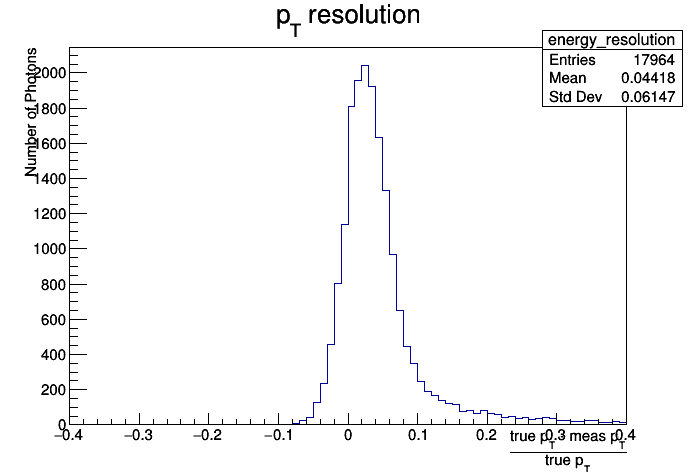
\includegraphics[width=0.49\textwidth]{energy_response_resolution__17g6a1_pthat2_clusterv1_small.png}
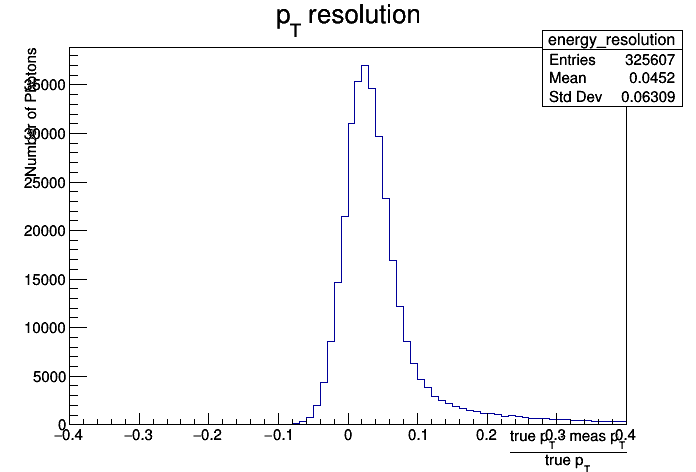
\includegraphics[width=0.49\textwidth]{energy_response_resolution__17g6a1_pthat2_clusterv2_small.png}
\caption{A 1-D projection of the v1 clusterizer's (left) and the v2 clusterizer's (right) $p_T$ response}
\label{fig:1D_pT_response_v1_vs_v2}
\end{figure}

Efficiency is measured by taking the ratio of the number of photons detected to the true number of direct photons. Once again, results produced by the 17g6a1 Monte-Carlo simulator are used for both the number of detected photons and the true number of photons. 

The following cuts are applied to the detected photon sample: photon $p_T$ $\>$ 10 GeV and the deep-photon output of Dr. Yue Shi Lai's neural net is cut to between 0.55 and 0.85. These are the same cuts that are used for the energy response. However, for the true photon sample, only the PDG code = 22 cut, which denotes a direct photon, is used because we want our efficiency to be the ratio of the number of photons detected, after all cuts, to the size of the entire sample of direct photons.

Efficiency is projected in two ways: as a 1-dimensional histogram with respect to photon $p_T$ and as a 2-dimensional histogram with respect to $\phi$ and $\eta$. In both cases, 2 histograms are taken, one of the number of measured photons projected over either $p_T$ or $\phi$ and $\eta$, and the other over the true number of direct photons projected over the same variable(s). The two histograms are then divided to produce the efficiency. The resulting histograms can be seen on Figure X.

It was found that the efficiency is negatively correlated with photon $p_T$, with an efficiency of about 20\% for a $p_T$ between 11 and 12 GeV and an efficiency of less than 1 \% for a $p_T$ between 19 and 20 GeV. The decrease in efficiency with increasing $p_T$ happens almost linearly, with the exception of photons with $p_T$ between 10 and 11 GeV, which have an efficiency of about 50\%. The overall efficiency was about 0.19 \% for both clusterizers. However, judging from the $\phi$-$\eta$ histograms, in those regions where most of the detectors are, and those that we concern ourselves with, the average efficiency was about 3.5 \% for both clusterizers, though the v1 clusterizer seemed to have had a far higher spread in efficiency than did the v2 clusterizer.

Thus, in conclusion, the v1 and v2 clusterizers seem to behave in essentially the same way with respect to energy response and efficiency, except that the spread over $\phi$ and $\eta$ of the efficiency is higher for the v1 clusterizer than it is for the v2 clusterizer and the v2 clusterizer has more data, by about an order of magnitude.

\begin{figure}
\includegraphics[width=0.32\textwidth]{efficiencies.png}
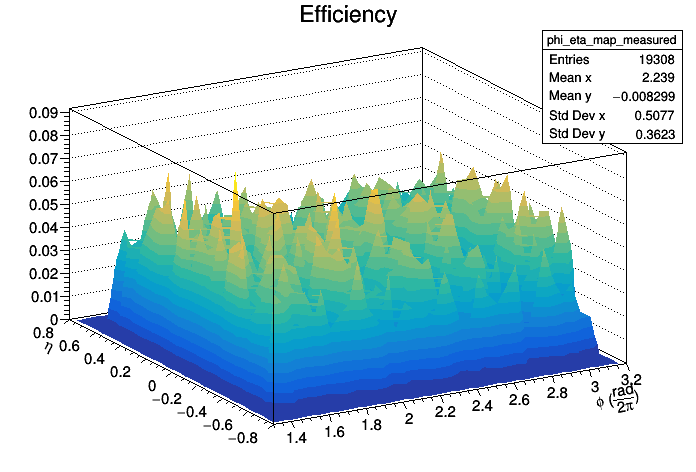
\includegraphics[width=0.32\textwidth]{efficiency_phietamap__17g6a1_pthat2_clusterv1_small.png}
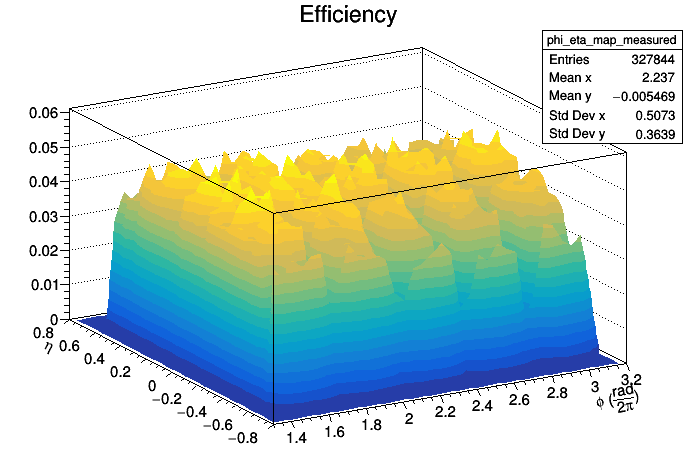
\includegraphics[width=0.32\textwidth]{efficiency_phietamap__17g6a1_pthat2_clusterv2_small.png}
\caption{From left to right: the efficiencies of the v1 and v2 clusterizers over photon $p_t$, the efficiency of the v1 clusterizer over $\phi$ and $\eta$, and the efficiency of the v2 clusterizer over $\phi$ and $\eta$}
\end{figure}
